\documentclass{standalone}
\usepackage{tikz}
\usetikzlibrary{patterns, positioning}
\usepackage[sfdefault]{ClearSans} %% option 'sfdefault' activates Clear Sans as the default text font
\usepackage[T1]{fontenc}

\begin{document}
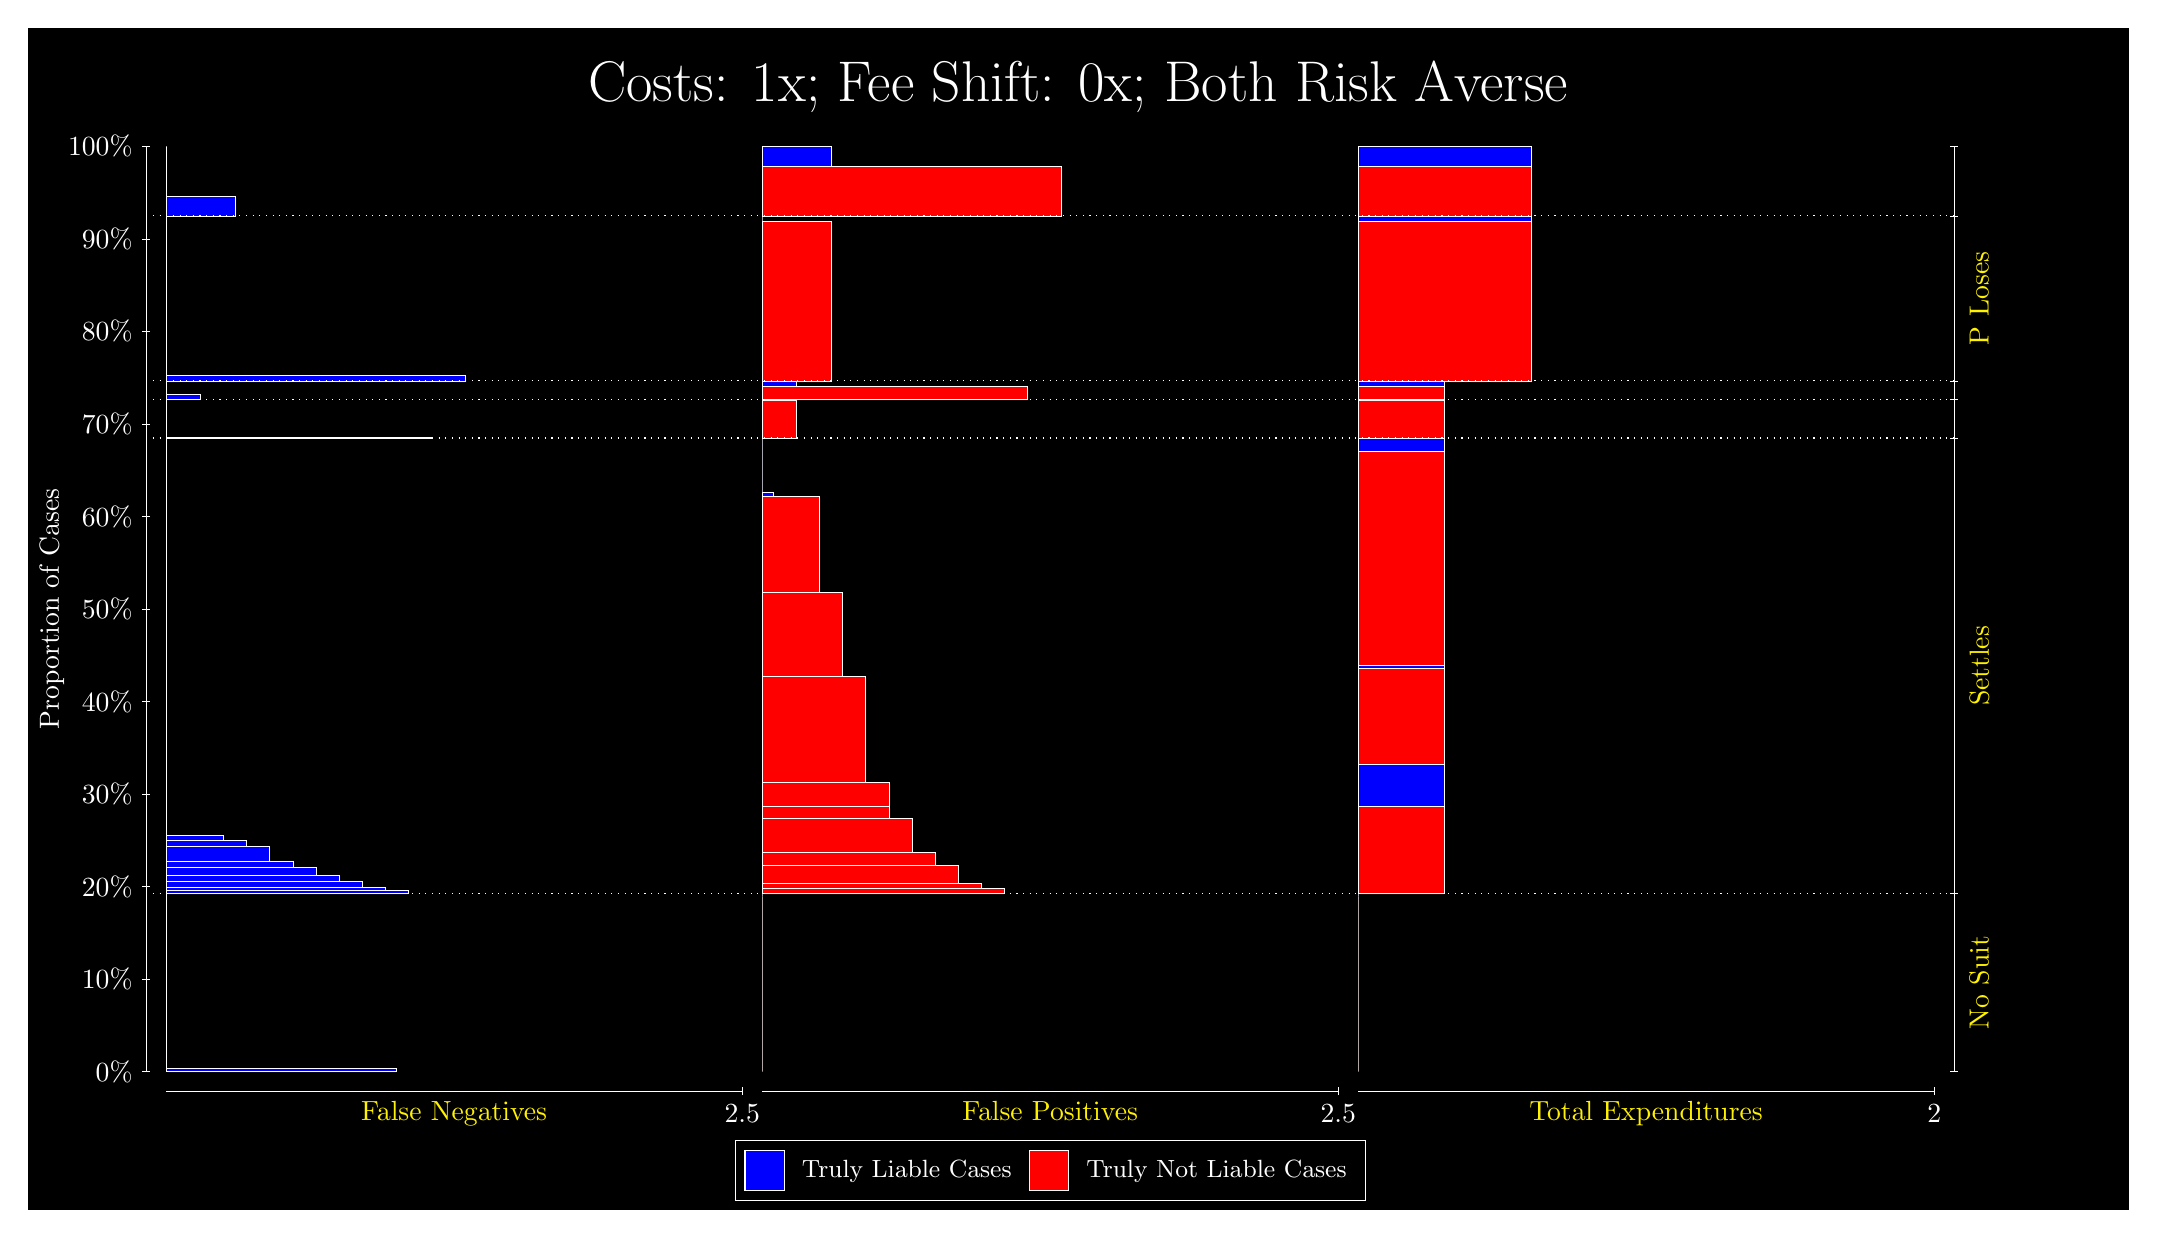
\begin{tikzpicture}
\draw[fill=black] (0,0) rectangle (26.667,15);
\draw[text=white] (0,13.5) rectangle (26.667,15) node[midway] {\huge Costs: 1x; Fee Shift: 0x; Both Risk Averse};
\draw[white, very thin] (1.5,1.75) -- (1.5,13.5);
\node[rotate=90, text=white, anchor=center] at (0.3, 7.625) {Proportion of Cases};
\draw[white, very thin] (1.45,1.75) -- (1.55,1.75);
\node[text=white, anchor=east] at (1.45, 1.75) {0\%};
\draw[white, very thin] (1.45,2.925) -- (1.55,2.925);
\node[text=white, anchor=east] at (1.45, 2.925) {10\%};
\draw[white, very thin] (1.45,4.1) -- (1.55,4.1);
\node[text=white, anchor=east] at (1.45, 4.1) {20\%};
\draw[white, very thin] (1.45,5.275) -- (1.55,5.275);
\node[text=white, anchor=east] at (1.45, 5.275) {30\%};
\draw[white, very thin] (1.45,6.45) -- (1.55,6.45);
\node[text=white, anchor=east] at (1.45, 6.45) {40\%};
\draw[white, very thin] (1.45,7.625) -- (1.55,7.625);
\node[text=white, anchor=east] at (1.45, 7.625) {50\%};
\draw[white, very thin] (1.45,8.8) -- (1.55,8.8);
\node[text=white, anchor=east] at (1.45, 8.8) {60\%};
\draw[white, very thin] (1.45,9.975) -- (1.55,9.975);
\node[text=white, anchor=east] at (1.45, 9.975) {70\%};
\draw[white, very thin] (1.45,11.15) -- (1.55,11.15);
\node[text=white, anchor=east] at (1.45, 11.15) {80\%};
\draw[white, very thin] (1.45,12.325) -- (1.55,12.325);
\node[text=white, anchor=east] at (1.45, 12.325) {90\%};
\draw[white, very thin] (1.45,13.5) -- (1.55,13.5);
\node[text=white, anchor=east] at (1.45, 13.5) {100\%};

\draw[white, very thin] (24.457,1.75) -- (24.457,13.5);
\draw[white, very thin] (24.407,1.75) -- (24.507,1.75);
\node[anchor=west] at (24.407, 1.75) {};
\draw[white, very thin] (24.407,4.0086) -- (24.507,4.0086);
\node[anchor=west] at (24.407, 4.0086) {};
\draw[white, very thin] (24.407,9.7959) -- (24.507,9.7959);
\node[anchor=west] at (24.407, 9.7959) {};
\draw[white, very thin] (24.407,10.287) -- (24.507,10.287);
\node[anchor=west] at (24.407, 10.287) {};
\draw[white, very thin] (24.407,10.522) -- (24.507,10.522);
\node[anchor=west] at (24.407, 10.522) {};
\draw[white, very thin] (24.407,12.616) -- (24.507,12.616);
\node[anchor=west] at (24.407, 12.616) {};
\draw[white, very thin] (24.407,13.5) -- (24.507,13.5);
\node[anchor=west] at (24.407, 13.5) {};

\draw[white, very thin, fill=blue] (1.75,1.75) rectangle (4.6775,1.7872);
\draw[white, very thin, fill=red] (1.75,1.7872) rectangle (1.75,4.0086);
\draw[white, very thin, fill=blue] (1.75,4.0086) rectangle (4.8239,4.0495);
\draw[white, very thin, fill=blue] (1.75,4.0495) rectangle (4.5312,4.0957);
\draw[white, very thin, fill=blue] (1.75,4.0957) rectangle (4.2384,4.1606);
\draw[white, very thin, fill=blue] (1.75,4.1606) rectangle (3.9457,4.2381);
\draw[white, very thin, fill=blue] (1.75,4.2381) rectangle (3.6529,4.3484);
\draw[white, very thin, fill=blue] (1.75,4.3484) rectangle (3.3602,4.4139);
\draw[white, very thin, fill=blue] (1.75,4.4139) rectangle (3.0674,4.6163);
\draw[white, very thin, fill=blue] (1.75,4.6163) rectangle (2.7746,4.6925);
\draw[white, very thin, fill=blue] (1.75,4.6925) rectangle (2.4819,4.7487);
\draw[white, very thin, fill=red] (1.75,4.7487) rectangle (1.75,9.7959);
\draw[white, very thin, fill=blue] (1.75,9.7959) rectangle (5.1167,9.8044);
\draw[white, very thin, fill=red] (1.75,9.8044) rectangle (1.75,10.287);
\draw[white, very thin, fill=blue] (1.75,10.287) rectangle (2.1891,10.353);
\draw[white, very thin, fill=red] (1.75,10.353) rectangle (1.75,10.522);
\draw[white, very thin, fill=blue] (1.75,10.522) rectangle (5.5558,10.593);
\draw[white, very thin, fill=red] (1.75,10.593) rectangle (1.75,12.616);
\draw[white, very thin, fill=blue] (1.75,12.616) rectangle (2.6283,12.869);
\draw[white, very thin, fill=red] (1.75,12.869) rectangle (1.75,13.5);
\draw[white, very thin, fill=red] (9.3189,1.75) rectangle (9.3189,3.9714);
\draw[white, very thin, fill=blue] (9.3189,3.9714) rectangle (9.3189,4.0086);
\draw[white, very thin, fill=red] (9.3189,4.0086) rectangle (12.393,4.0716);
\draw[white, very thin, fill=red] (9.3189,4.0716) rectangle (12.1,4.1437);
\draw[white, very thin, fill=red] (9.3189,4.1437) rectangle (11.807,4.3716);
\draw[white, very thin, fill=red] (9.3189,4.3716) rectangle (11.515,4.5367);
\draw[white, very thin, fill=red] (9.3189,4.5367) rectangle (11.222,4.9724);
\draw[white, very thin, fill=red] (9.3189,4.9724) rectangle (10.929,5.1208);
\draw[white, very thin, fill=red] (9.3189,5.1208) rectangle (10.929,5.421);
\draw[white, very thin, fill=red] (9.3189,5.421) rectangle (10.636,6.7713);
\draw[white, very thin, fill=red] (9.3189,6.7713) rectangle (10.344,7.8346);
\draw[white, very thin, fill=red] (9.3189,7.8346) rectangle (10.051,9.0558);
\draw[white, very thin, fill=blue] (9.3189,9.0558) rectangle (9.4652,9.112);
\draw[white, very thin, fill=blue] (9.3189,9.112) rectangle (9.3189,9.7959);
\draw[white, very thin, fill=red] (9.3189,9.7959) rectangle (9.758,10.278);
\draw[white, very thin, fill=blue] (9.3189,10.278) rectangle (9.3189,10.287);
\draw[white, very thin, fill=red] (9.3189,10.287) rectangle (12.686,10.456);
\draw[white, very thin, fill=blue] (9.3189,10.456) rectangle (9.758,10.522);
\draw[white, very thin, fill=red] (9.3189,10.522) rectangle (10.197,12.546);
\draw[white, very thin, fill=blue] (9.3189,12.546) rectangle (9.3189,12.616);
\draw[white, very thin, fill=red] (9.3189,12.616) rectangle (13.125,13.248);
\draw[white, very thin, fill=blue] (9.3189,13.248) rectangle (10.197,13.5);
\draw[white, very thin, fill=red] (16.888,1.75) rectangle (16.888,3.9714);
\draw[white, very thin, fill=blue] (16.888,3.9714) rectangle (16.888,4.0086);
\draw[white, very thin, fill=red] (16.888,4.0086) rectangle (17.986,5.1208);
\draw[white, very thin, fill=blue] (16.888,5.1208) rectangle (17.986,5.647);
\draw[white, very thin, fill=red] (16.888,5.647) rectangle (17.986,6.8682);
\draw[white, very thin, fill=blue] (16.888,6.8682) rectangle (17.986,6.9091);
\draw[white, very thin, fill=red] (16.888,6.9091) rectangle (17.986,9.6229);
\draw[white, very thin, fill=blue] (16.888,9.6229) rectangle (17.986,9.7959);
\draw[white, very thin, fill=red] (16.888,9.7959) rectangle (17.986,10.278);
\draw[white, very thin, fill=blue] (16.888,10.278) rectangle (17.986,10.287);
\draw[white, very thin, fill=red] (16.888,10.287) rectangle (17.986,10.456);
\draw[white, very thin, fill=blue] (16.888,10.456) rectangle (17.986,10.522);
\draw[white, very thin, fill=red] (16.888,10.522) rectangle (19.083,12.546);
\draw[white, very thin, fill=blue] (16.888,12.546) rectangle (19.083,12.616);
\draw[white, very thin, fill=red] (16.888,12.616) rectangle (19.083,13.248);
\draw[white, very thin, fill=blue] (16.888,13.248) rectangle (19.083,13.5);
\draw[white, dotted] (1.5,4.0086) -- (24.457,4.0086);
\draw[white, dotted] (1.5,9.7959) -- (24.457,9.7959);
\draw[white, dotted] (1.5,10.287) -- (24.457,10.287);
\draw[white, dotted] (1.5,10.522) -- (24.457,10.522);
\draw[white, dotted] (1.5,12.616) -- (24.457,12.616);
\draw[white, very thin] (1.75,1.5) -- (9.0689,1.5);
\node[text=yellow, anchor=north] at (5.4094, 1.5) {False Negatives};
\draw[white, very thin] (9.0689,1.45) -- (9.0689,1.55);
\node[text=white, anchor=north] at (9.0689, 1.45) {2.5};

\draw[white, very thin] (9.3189,1.5) -- (16.638,1.5);
\node[text=yellow, anchor=north] at (12.978, 1.5) {False Positives};
\draw[white, very thin] (16.638,1.45) -- (16.638,1.55);
\node[text=white, anchor=north] at (16.638, 1.45) {2.5};

\draw[white, very thin] (16.888,1.5) -- (24.207,1.5);
\node[text=yellow, anchor=north] at (20.547, 1.5) {Total Expenditures};
\draw[white, very thin] (24.207,1.45) -- (24.207,1.55);
\node[text=white, anchor=north] at (24.207, 1.45) {2};

\node[text=yellow, centered, rotate=90] at (24.777, 2.8793) {No Suit};
\node[text=yellow, centered, rotate=90] at (24.777, 6.9023) {Settles};


\node[text=yellow, centered, rotate=90] at (24.777, 11.569) {P Loses};


\draw (12.978300999999998,1.5) node[draw=none] (baseCoordinate) {};
\begin{scope}[align=center]
        \matrix[scale=0.5, draw=white, below=0.5cm of baseCoordinate, nodes={draw}, column sep=0.1cm]{
            \node[rectangle, draw, minimum width=0.5cm, minimum height=0.5cm, fill=blue] {}; &
            \node[draw=none, font=\small, text=white] (B) {Truly Liable Cases}; &
            \node[rectangle, draw, minimum width=0.5cm, minimum height=0.5cm, fill=red] {}; &
            \node[draw=none, font=\small, text=white] (B) {Truly Not Liable Cases}; \\
            };
\end{scope}

\end{tikzpicture}
\end{document}